\documentclass[]{report}   % list options between brackets
\usepackage{fullpage}
\usepackage[top=0.75in, bottom=0.75in, left=1.25in, right=0.75in]{geometry}
\usepackage{setspace}
\usepackage{array}
\usepackage[pdftex]{graphicx}
\usepackage{subfig}
\usepackage{multirow}
\usepackage{hyperref}
\usepackage{url}
\usepackage{titlesec}
\usepackage{cite}
\usepackage{booktabs}
\usepackage[numbers]{natbib}
\usepackage{fancyvrb}
% type user-defined commands here
\doublespacing
\titleformat{\chapter}[hang]{\bfseries\huge}{\thechapter.}{2pc}{}
\begin{document}

\title{Gesture recognition\\ in motion captured data \\using Hidden Markov Models\\\\\\}   % type title between braces
\author{Sharon Lourduraj\\993833107\\\\M.Eng Report\\\\\\\\University of Toronto\\Mechanical and Industrial Engineering}         % type author(s) between braces
\date{Jan 12, 2011}    % type date between braces
\maketitle

\begin{abstract}
Hidden Markov Models (HMMs) lend themselves well in a variety of applications that are dependent on spatio-temporal variability; gesture recognition is one such application. This report details the experimental process of constructing, and optimizing a HMM framework for body pose gesture recognition. A gesture recognition rate of 63\% for an acted data set is achieved and a recognition rate of 60\% for an un-acted data set is achieved. In the experiments, motion capture data is used as a primary means for posture tracking, than the traditional image sequences. An experiment that used Xbox Kinect to capture and tracking body postures was also conducted, yielding similar results in recognition.

\end{abstract}
\tableofcontents
\chapter{Introduction}             % chapter 1
Technologies as we know, from our hand-watches to parts for space stations, are built by automated machines on a daily basis. Today, it is an important part of our lives. And in the future it will be even more important as we start interacting with intelligent agents to accomplish our tasks. The key difference between today's robots and tomorrow's robot is not the computing power or sensing capabilities, it will be their seamless interaction with their users. A robot that manufactures parts for automobiles certainly does not need to be socially friendly with its human operators. These robots do what they are told, without question. But we want to look into robots that might one day service users, help you make coffee, assist someone in a grocery store, help children cross traffic lights, be a friendly companion, act as a guide dog, or help elders in need around the house. These robots are not performing tedious tasks on a daily basis, but are being interactive with humans, and able to socialize with them. For this to happen, robots need to sense and interpret human interaction, their gestures and body language.

A human expressing a gesture through body language, goes through a sequence of observable postures. These observations can be discretized to extract a smaller subset of postures through which a gesture can be conveyed. Think of it as watching a movie. If we drop the frame-rate significantly we can still visually interpret the movie. The order in which each observation occurs is of importance, shifting the observation's order in the sequence would convey a completely different gesture. Expression of a gesture also varies from person to person; it also varies depending on the context that someone is experiencing.

We introduce the problem of recognizing gestures from data obtained by motion capture systems. Many methods exists in recognizing gestures\cite{4154947, Yang_1994_329}, template-matching, dictionary lookup, statistical matching, neural networks, and other ad hoc methods. Some techniques are widely applicable to various problems in gesture recognition while others are designed specifically to resolve a particular problem. Gesture recognition is considered to have stochastic properties\cite{Yang_1994_329}, as such a technique that uses the stochastic nature of the problem to its advantage would be of value.

A Hidden Markov Model (HMM) is defined as a doubly stochastic process with an underlying stochastic process that is not observable (it is hidden), but can only be observed through another set of stochastic processes that produce the sequence of observed symbols\cite{1165342}. Being robust to adapt to spatio-temporal variability\cite{springerlink:10.1007/s00422-004-0516-0}, HMMs lend themselves well to the task of gesture recognition.

This report is an account of the experimental steps taken in using HMMs to recognize gestures in 3D motion captured data. For a full mathematical account of HMM, \citet{1165342} is a great source of information. The initial experiments focused on discovering the process involved in using HMMs to train and classify motion capture data. The later experiments focus on improving the performance of HMM to provide better results. Finally, we test the robustness of the HMM framework by using a different dataset than the one which was used to develop the framework. We also perform an experiment using Xbox Kinect to capture body postures performed by an actor, and classify them.

The primary purpose of these experiments is to implement a body gesture tracking and recognition feature onto a socially assistive robot named Brian, from the University of Toronto's Autonomous Systems and Biomechatronics Lab. Brain is an assistive robot with human-like demeanors, and human affective intent recognition, identification and decision making abilities capable of natural and believable social interaction via verbal and non-verbal communication\cite{dmcoll}. It is especially designed to be socially assistive with the elderly who are diagnosed with cognitive impairment.
Research has already been done to recognize and classify body postures in Brian, using a unique non-contact and non-restricting automated sensor-based approach for identification and categorization of human upper body language\cite{dmcoll}. In this paper we hope to provide insight into recognizing and classifying a sequence of body postures to determine the emotion being experienced by the user.

\section*{Outline}
We introduce the overall gesture recognition process using HMMs in Chapter \ref{sec:overllprocess} with a summary of some of the works consulted. Chapter \ref{sec:fwc} outlines the main components of the process whose considerations are invaluable in making decisions to improve gesture recognition performance. Chapter \ref{sec:results} discusses the results of the experiments conducted, and analyzes the various pitfalls encountered in building a system to achieve a 63\% recongition rate from data sets in literature, and a 75-80\% recognition rate on an experiment performed using a Xbox Kinect to classify simple motions.

\chapter{Gesture Recognition with HMM}\label{sec:overllprocess}
We discuss the details of the gesture recognition process using HMM in this chapter. This will put the reader in perspective of the various parts that work together in using HMMs for gesture recognition. Due to the generality of the HMM algorithm it can be applied to any problem, in any domain, that can be translated into entities that a HMM process can take advantage of.

\section{Works consulted}
\citet{Fong2003143} conducted a survey of socially-interactive robots providing us with sufficient history and knowledge into the applications such robots. The paper also discusses the various design considerations such as robot embodiment, emotion sensing and emotion as a control mechanism, speech, facial expressions, body language, personality traits, and the various forms of human-oriented perception. A key point is noted in the paper in regards to having meaningful interactions with humans. Social robots must perceive the world as humans do, that is sensing and interpreting the same phenomena that humans observe \cite{Fong2003143}. It is identified that perceptual abilities similar to humans are necessary in addition to the sensing capabilities required for conventional functions. People tracking, speech recognition, gesture recognition and facial perception are some of the human-oriented perceptual abilities listed.

The purpose of the experiment was to implement and evaluate the use of HMMs to train and classify sequence of postures in motion captured data. HMMs can be applied to any problem where spatio-temporal variability is of importance\cite{ 1165342}. The implementation of HMM as a machine learning algorithm is straight forward and explained by \citet{ 1165342}. HMMs can virtually be applied to any domain; applications include speech recognition\cite{54527}, hand writing recognition\cite{541414}, data mining\cite{5602641}, image classification\cite{4379516}, and of course gesture recognition\cite{4154947}. 

In almost all of the works the implementation of the HMM algorithm remains the same. The difference between the various works is that they innovate in the extraction of feature vectors from an acted gesture. \citet{Huang:2001:MHG:375397.375409} propose a feature extraction by a hybrid technique combining the spatial and the temporal information of each frame to extract the feature images. \citet{springerlink:10.1007/s00422-004-0516-0} introduce a technique of template matching to generate observation symbols using a Johansson display that encodes the motion of a moving person. \citet{799904} introduce a HMM-based threshold model that rejects input patterns which are recognized as non-gesture motions. \citet{Chen2003745} introduce a method to recognize continuous gestures with a stationary background. \citet{840674} extract features by tracking the skin-color blobs corresponding to the hand into a body-face space centered on the face of the user\cite{840674}. \citet{Rigoll98highperformance} propose feature vectors based on global motion features, extracted from each difference image of the image sequence. \citet{Pellegrini06humanposture} use stereo vision sensors to track posture, and then match against the 3D model of a human to extract feature vectors, such as hip angle, and knee angle. 

Feature vectors improve the recognition accuracy of the HMM in a specific problem domain, works exist that show how HMM can be used in applications that use gesture recognition. \citet{4755984} demonstrate the application of imitating a human's motion by a humanoid through a motion capture system. They use a variation based on HMMs to learn, recognize and generate motion. \citet{Starner95visualrecognition} demonstrate how HMMs can be used to recognize American Sign Language. Similarly, codebook creation plays an important role as we discovered while performing the experiments. \citet{springerlink:10.1007/s00422-004-0516-0} and \citet{springerlink:10.1007/11492429_73} demonstrate the use of template database as a codebook. While, \citet{Yang_1994_329} demonstrates a traditional approach of using k-means algorithm to cluster and quantize data into a codebook.

The initial experiments were performed on the data set from \citet{Kleinsmith:2006:CDR:1221613.1222203}. And a final experiments were conducted on a different data set from \citet{KlEINSMITH_Bianchi-Berthouze_Steed_2011}. Though they employed neural networks as the machine learning framework to train and recognize gestures, their work was significant in understanding proper selection of feature vectors. They also detail the use of 3D motion capture data directly for affective posture recognition. Their works demonstrate how an emotion is conveyed by different cultures, and the various emotions that people portray when they are performing a task naturally. 

We also looked into some literature regarding gesture classification using means other than HMMs. \citet{Caridakis201052} take advantage of the clustering properties of Self-Organizing Maps for gesture recognition; as self-organizing feature maps lead themselves well to model spatio-temportal information extracted from images. \citet{Oz20111204} use artificial netural networks for gesture recognition in American Sign Language, where data is captured via a sensory glove. The bibliography section of the report includes many more works that were consulted to gather knowledge about gesture recognition and HMMs in general. 

\section{Terms}
For clarity we establish some terms and their relative meaning, strictly as we have used them in this report and in our experiments.
\begin{description}
  \item[Feature Data] A specific property of a feature on a person's body, such as the position of the wrists, angle between the elbows, angle at the knees, or the position of the left-side of the head. 
  \item[Posture] A posture is made up of a group of feature data. Together, they establish a person's pose. 
  \item[Gesture] A gesture is made up of many postures. When one or more postures are executed in a sequence they convey a message from the person to an observer.
  \item[Emotion] An emotion categorizes a group of gestures together. All gestures that indicate that a person is angry would fall under the angry emotion.
\end{description}

We call the data captured from the motion capture system a \texttt{gesture}, which is a specific instance of an \texttt{emotion}. When one or more gestures are similar to each other they fall under the same emotion. For example, being \texttt{angry} is an emotion, but one can show anger through various gestures. The data from the motion capture system is a sequence of frames with pose data (angles, or position of body points in space). A \texttt{posture} is a specific frame in a gesture. A gesture is made up of a sequence of postures, as shown in figure \ref{fig:fw1}.

\begin{figure}[htbp]
	\centering
		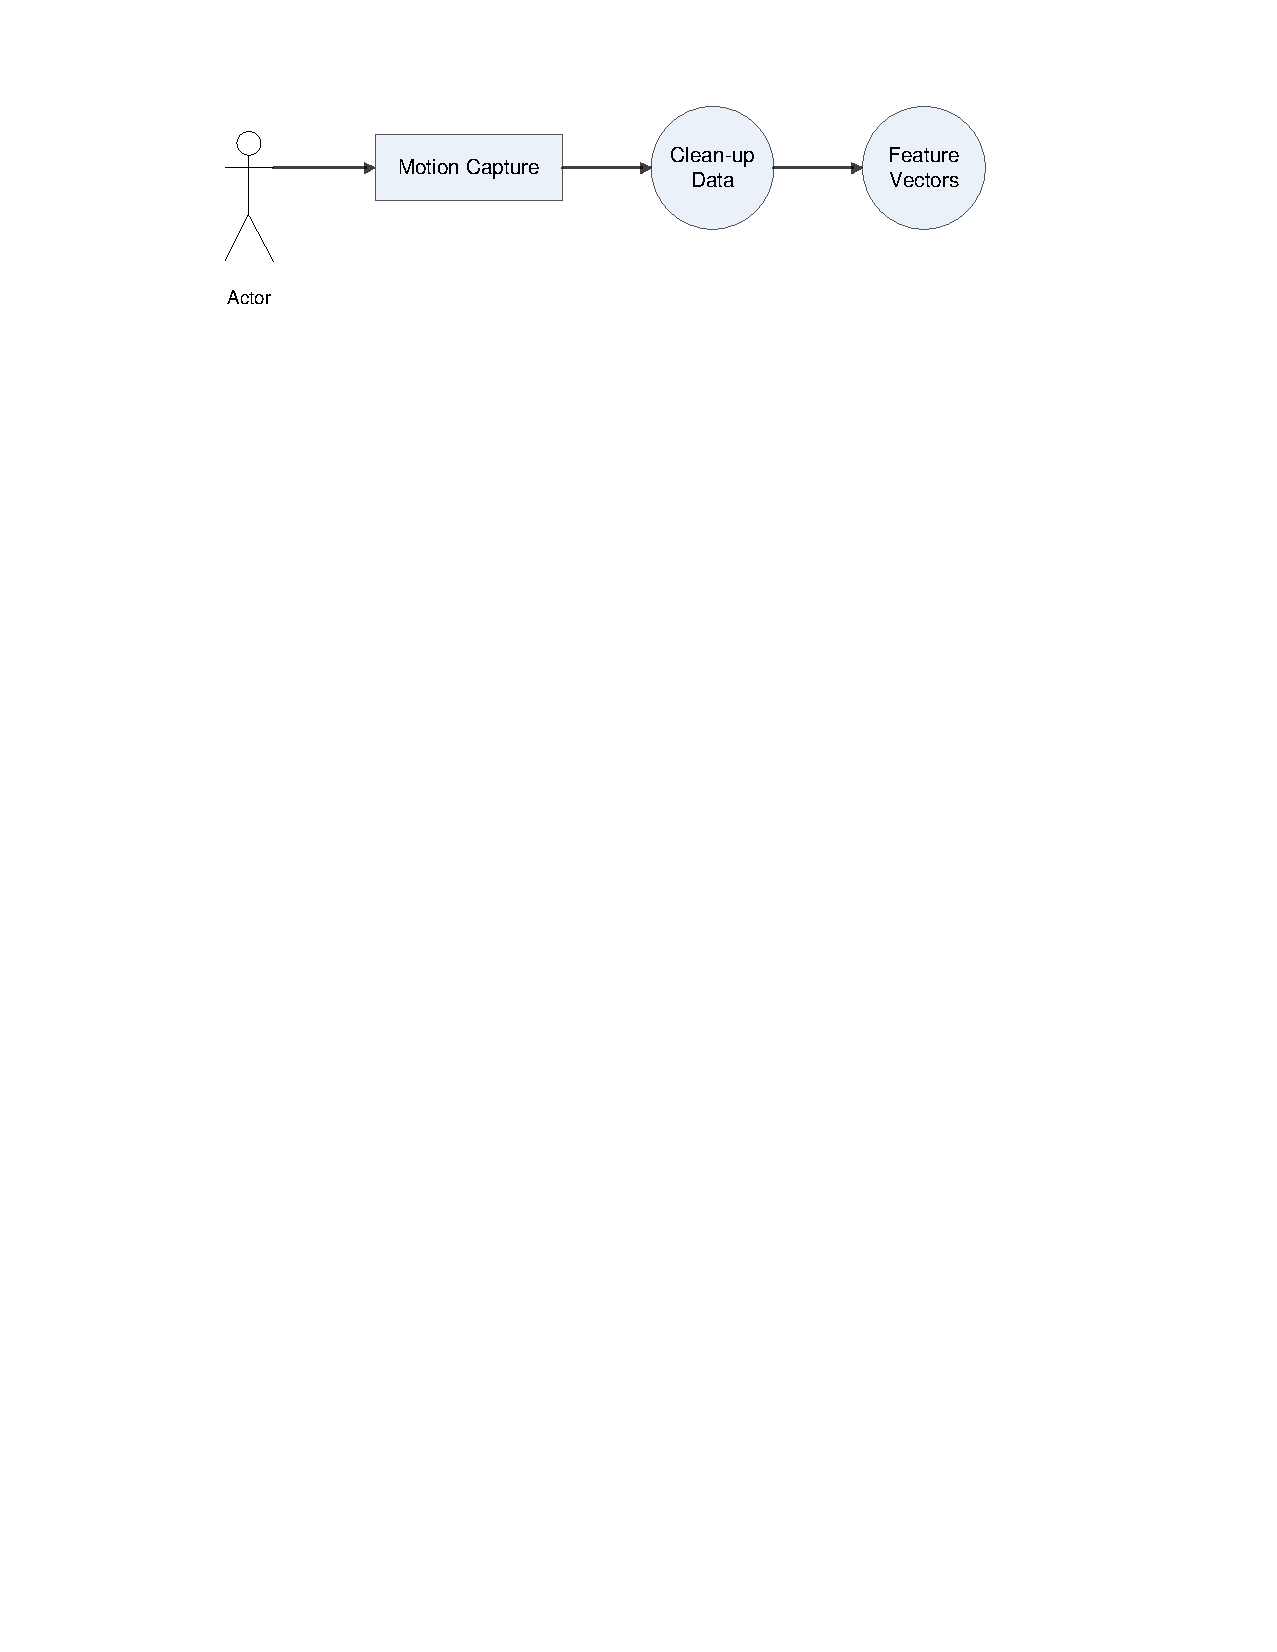
\includegraphics{fw1.pdf}
	\caption{Gestures, postures and features from motion capture data.}
	\label{fig:fw1}
\end{figure}

\section{Data set}
As in any machine learning algorithm, a data set plays an important role in enabling the algorithm to train, classify and re-train. There are two basic ways through which data can be captured for gesture recognition, data captured through a video camera, and data captured through a 3D marker tracking system\cite{dmcoll}. The camera captures a sequence of images that is used to extract features later in the process. The sophistication, or the details, of the data captured is reliant on the camera itself. A hi-definition camera would capture more details versus a low definition camera; likewise a camera that is able to collect color data can provide additional details of the scene.

A 3D marker tracking system is a sophisticated derivative of using a video camera to capture data. Rather than capture details of the scene, the system captures movements of an actor's skeletal features. This is done by having many video cameras positioned at significant locations. These are then used to track markers on an actor wearing a specialized suit. Markers are positioned appropriately at significant locations such as wrists, knees, head, waist, spine, hips and many more. An algorithm then interprets the data from the various cameras and transforms them into position coordinates as it corresponds to the human skeletal frame. In essence, a single frame of this transformed data is a posture as defined earlier. This data can be further processed into rotation angles, or Euler angles corresponding to a datum, as necessary.

\citet{Morie200731} provides a summary of their experiments in a creating a markerless visual tracking system inspired by the brain; for face and object recognition. Another example of a markerless 3D posture tracking system is the use of Microsoft Xbox Kinect \cite{Kar_2010}. Regardless of how the data is captured, for gesture recognition a data set contains a collection of gesture movies. Dissecting further, a movie contains a sequence of frames; in our case a gesture movie contains a sequence of posture frames. And each posture frame contains data related to a feature that was tracked. The differences between the various tracking mechanism narrows down to the posture frame. A simple video capture system records raw light data of the scene in each frame, while a 3D marker motion capture system captures joint locations or angles in each frame. A raw data would need to be processed further to extract the required features; in fact, any data can be processed further to refine features necessary to accomplish gesture tracking and recognition. 

\section{Feature Vector}
The next step in the process is to extract feature vectors. Feature vectors isolate the necessary data from the redundant and non-essential data; data related to the scene from data related to the actor's limb positions. This is one of the more involved steps in the process. Every machine learning algorithm relies on feature vectors for training and classification, so does HMM. The feature extraction process can vary from being very simple to being extremely complex. Feature vectors are extracted from a posture or across multiple postures. The feature, location of the actor's head can be extracted from the posture, while the velocity of the actor's head needs to be extracted across two postures over time. A posture can have multiple features, combined they are called feature vectors. For a gesture containing 500 frames (postures), 500 feature vectors can be derived. The dimension of a feature vector is dependent on the number of the features. A feature can have multiple dimensions; location of the actor's wrist has three dimensions in space, while the actor's elbow angle has only one dimension (the angle itself).  This process is repeated for all the gestures captured.

Features that are to be extracted depend on the data representation in the data set. A 3D marker based motion capture system provides the information of spatial coordinates in all three planes. Spatial coordinates are not the only data about a feature that can be extracted; much other information can be extracted for a feature, some can even define complex relationships between sequences of postures. Applying a difference operator to two posture frames would give us velocity feature vectors. Having spatial coordinates of various features allows us to calculate other information easily, such as head tilt angle, direction of head, angle at the elbow, and depth of each wrist. On the other hand, obtaining such information from a 2D video camera is not straight forward. To extract such information from a 2D image one needs to apply image processing techniques\cite{springerlink:10.1007/978-3-642-04229-4_4}. Typically, this would involve normalizing the image, then extracting the actor from the image, and then finally perform a template analysis to extract data from the image. One can even calculate the average movement of pixels in a 2D image to estimate motion of a specific feature in that gesture\cite{Rigoll98highperformance}.

Feature vectors can be anything from the posture frame that is calculate-able, quantize-able and provides relevant information about the data that is going to be trained. Specific examples include, position coordinates, velocity, acceleration, angular velocity and angular acceleration of any number of features that are necessary to accomplish the training of a gesture and provide accurate classification. Figure \ref{fig:fv1} highlights some feature that were used in tracking and classification of a \texttt{Happy} gesture. Suppose we have a gesture where the actor is hopping in the air, we should extract feature data corresponding to the position and velocity of knees, ankles and angle at the knees for a system to train and recognize a related gesture accurately. Ignoring a feature could result in misclassification.

\begin{figure}[htbp]
	\centering
		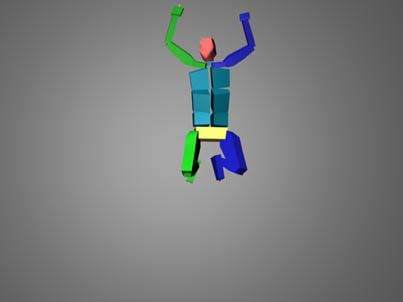
\includegraphics[scale=0.5]{aff2.jpg}
	\caption{Example of feature vectors in a posture frame\cite{Kleinsmith:2006:CDR:1221613.1222203}}
	\label{fig:fv1}
\end{figure}

The feature extraction process does impose a significant overhead in the training and recognition process, suppose if the camera were to provide us with 10 images per second, then we would have to isolate and calculate 10 frames in less than one second to keep up with incoming data. Depending on the resolution of the data, the number of features, and the complexity of features to be extracted, this overhead could either increase or decrease.
 
\section{Codebook}
Once the feature vectors are extracted from the data sets, a codebook needs to be created. This is an abstraction layer that separates the problem domain from the mathematics involved in HMM. Templates need to be extracted from these feature vectors. Templates are just a mechanism to group similar postures together. If someone is raising their hand, we can take three snapshots while this action takes place; when their hand is at the initial position, when the hand moves half way up, and then at the final position. Any intermediate snapshot is unnecessary as the three snapshots are enough to convey that the person is raising their hand. Thus, given a set of feature vectors from the many gestures to be trained, we identify few templates from it that would best represent the gestures that need to be classified. Note that templates from one gesture can be used in another gesture; hence the template dataset is essentially a database of unique postures. The existing postures in the template database can also be used to create other gestures, or variation of the particular gesture. This introduces the idea of a \texttt{codebook}, a synonym for a template database. We label each posture in the codebook with a unique number from $1\ldots n$, and one can refer to them with a page number. In HMM terms, the page number, or a referring id, is known as an observation \texttt{symbol}.

Consider a gesture and a codebook; we need to transform each posture in the gesture into a symbol in the codebook. Thus rather than having a $n\times m$ matrix of postures and features, we have a $1\times m$ vector where each column corresponds to a symbol in the codebook. Note that there is a loss of information in this transformation. The original gesture file contains accurate information about the gesture, while the codebook transformed version contains an approximate, hopefully sufficient, version of the gesture due to quantization. The concept of codebooks is necessary to work with HMMs, as HMMs are built around the concept of states and observations. We discuss briefly about states and observations in the following section. 

\begin{figure}[htbp]
	\centering
		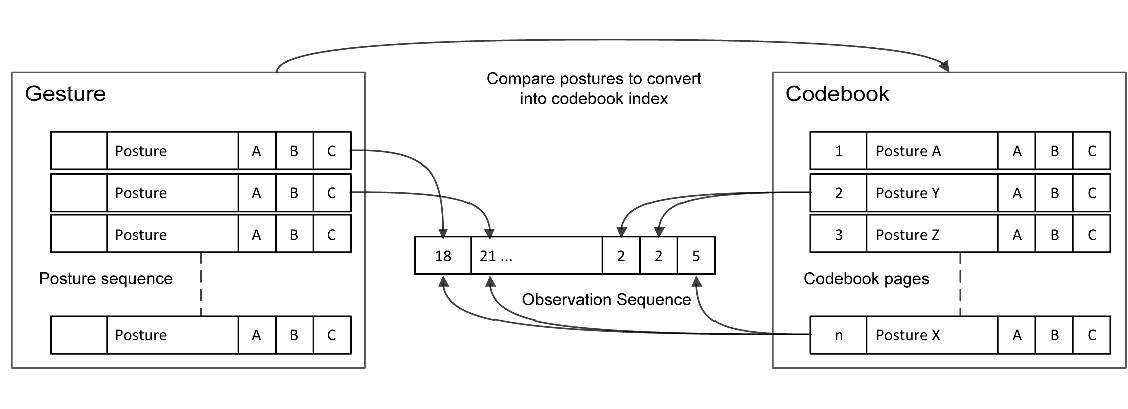
\includegraphics[width=1.0\textwidth]{fw2.pdf}
	\caption{Observation sequence of a gesture determined from a codebook.}
	\label{fig:fw2}
\end{figure}

\section{Observations sequences and states}
With the codebook created, we are now able to transform a sequence of input frames with rich posture data into a sequence of symbols, which approximates the input sequence, from the codebook. This input sequence is known as the observation sequence; indicating that the system observes the occurrences of symbols in the codebook as the gesture is taking place. Figure \{fig:fw2} shows how a gesture input (a sequence of posture frames) is converted into an observation sequence. Every input posture frame in the gesture is converted into a feature vector. This conversion allows us to compare features from a posture to the stored features from the templates in the codebook. The symbol for the closest matching template is obtained. Thus, we generate the observation sequence by obtaining the corresponding symbols from the codebook. The numerical order of the sequence itself is irrelevant as they are only a reference to the location of the template in the codebook.

The order of the symbols in the sequence of observations matter; changing the order of the symbols in the sequence would imply a very different gesture or emotion. As such, each observation sequence is said to occur at specific arbitrarily defined states in a gesture. A gesture can have many states depending on the complexity of the gesture. Similar to \citet{Yang_1994_329} we assume the gestures to have three observable states, a ready state, an intermediate state and a distinctive state. Between these states there are many hidden states, or transition states, that we cannot visibly distinguish as an observer. If we consider someone giving a wave, there are three visible poses we notice. The ready state where the hands are relaxed, the intermediate state where the hands are bent in front of the person, and the distinctive state where the person has their palm open and tilted about the wrist. However, one can convey a hand wave with two postures, a posture with the wrist tilted to the left and a posture with the wrist titled to the right. With this interpretation we cannot say that a gesture must have three distinct states; namely a ready state, an intermediate state or a distinctive state. A gesture is considered to have temporal properties \cite{Wilson96recoveringthe} because gestures consists of a sequence of poses across time. This leads us to the conclusion that states are hidden and non-observable. States maybe hidden but we can observe the output of those states, the postures that each state emits. And a HMM can determine some information about the states through a sequence of observations\cite{1165342}. This is why Hidden Markov Models are applicable for gesture recognition; they expose hidden states through the observation patterns given as an input. The number of states is optimized through experimentation of various gestures. Different gestures can have different states, and certain states improve the accuracy of using HMMs to classify similar gestures. 

\section{Training and Classification}
A HMM is trained by providing a sequence of observations, symbols from the codebook. However, it is unaware of the posture that a symbol represents. Mathematically, a state has a probability distribution for each observation. The task of training calculates the maximum likelihood estimate of the parameters that best represent the probability distributions\cite{1165342}. The parameters obtained are the state transition probability matrix and the emission probability matrix. The state transition probability matrix dictates the likelihood of the transition from one state to another, while the emission probability matrix calculates the likelihood of an observation occurring given a particular state. The Baum-Welch algorithm \cite{1165342} calculates the local maximum likelihood estimates given an observation sequence. 

\begin{table*}[htbp]
	\centering
		\begin{tabular}{|l|c|c|c|c|}
		\hline
             & State 1 & State 2 & State 3 \\ \hline
        State 1 & 0.183     & 0.196    & 0.621    \\ \hline
        State 2  & 0.256     & 0.744    & 1.3e-05      \\ \hline
        State 3 & 0.999    & 2.2e-17    & 3.1e-05     \\ \hline
		\end{tabular}
	\caption{State transition matrix for a 3-state HMM.}
	\label{tab:hmm3state}
\end{table*}

Given an observation sequence to train a HMM for, the Baum-Welch algorithm is a convergence algorithm that begins the likelihood estimation process with a randomized\cite{Stamp04arevealing} initial state transition probability, and emission probability matrix. An example of a transition probability matrix is shown in table \ref{tab:hmm3state}. The algorithm iteratively improves the maximum likelihood of the occurrence of the observation sequence, until the probability matrices reach a maxima. When we train a HMM for an input gesture, the postures in the gesture are converted to observation symbols. And they are then given as inputs to the training algorithm. The probability matrices encode the occurrence of the observation symbols for a given gesture\cite{Yang_1994_329}. Many gestures can be trained under the same HMM as well. When another observation sequence is provided to the algorithm for training under the same HMM, the already existing probability matrices are used as a starting point. The matrices are then optimized for the occurrence of the new observation sequence as well.

For classification, motion from the actor is captured in a similar manner that is used to create a training data set, as discussed in previous sections. The captured motion is processed and converted to a sequence of posture frames, which is then translated into a sequence of codebook symbols by comparing the feature data. This is known as the observation sequence, which serves as an input to a HMM for classification. 

Suppose we have a HMM that is trained to recognize the hand wave gesture, and an observation sequence of someone waving their hand is provided. The HMM would return an estimate for the occurrence of the postures (observations) in the input gesture. The question then becomes, does the given sequence of observation make sense for it to be classified as a hand wave? If the answer is yes then the gesture is classified as a hand wave. A HMM returns a likelihood estimate of the input sequence occurring\cite{1165342}, based on the training provided. If the estimate is high then we consider the input sequence to contain the said gesture, otherwise it is classified as some other gesture. As in figure \ref{fig:fw3}, by evaluating the same sequence of inputs in parallel with other trained HMMs, we can obtain their corresponding likelihood estimates for each HMM. We then select the best HMM for the input sequence to belong to by analyzing the likelihood estimates, and classify it under the corresponding gesture label.

\begin{figure}[htbp]
	\centering
		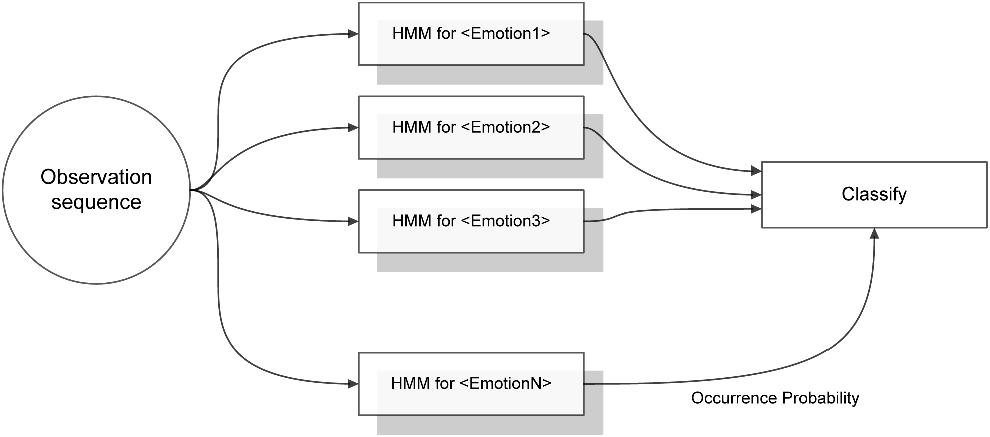
\includegraphics[width=0.90\textwidth]{fw3.pdf}
	\caption{Classifying an observation sequence with multiple HMMs.}
	\label{fig:fw3}
\end{figure}

\chapter{Framework Components}\label{sec:fwc}
Three principle components were considered when making decisions on improving performance and accuracy of the gesture recognition framework, HMM topology, feature vectors, and codebook selection. Based on experiential evidence through the learning and discovery, that was involved in implementing and running these experiments, it can be said that the HMM topology and feature vectors play a key role in the performance and accuracy of using any HMM. This chapter discusses some of the points that were considered when performing the experiments.

\section{HMM topology}
A HMM Topology describes how the various states could be related to one another. Mathematically, this is described by the probability distribution from one state to another. Keeping in mind the problem of recognizing body gestures while performing an activity, if we consider the emotion of being \texttt{angry}, there are various transitions that a body goes through to exhibit an angry gesture.

\citet{Yang_1994_329} and \citet{4755984} discuss simple HMM network architectures as discussed here in their research implementation of gesture recognition in hand gestures, and human motion imitation respectively. While \citet{springerlink:10.1007/11492429_73} outline a unique multi-tier HMM topology, where one HMM is trained for every gesture, and then they are all combined together into a single HMM, for their experiment in gesture based robot motion control. Considering the simplest case of the angry gesture from a T-posture, first the arms bend in toward the hips, the legs spread apart and finally the hands rest on the hips. These sequence of states indicate that the person is at an \texttt{angry} emotional state. This is a linear progression of states, a visualization is shown in figure \ref{fig:lineartopology}. The numbers in the figure indicate a posture from the respective codebook page, and the sequence of numbers combined together conveys a specific gesture. If the hands are rested on the hips before the legs are spread apart then the sequence of events most likely does not indicate an angry emotion. If one were to train a generic HMM to classify the angry gesture the probability distribution would force the HMM into a linear topology. The left-right linear topology is perfect for recognizing a gesture that is progressive in nature. There are various kinds of angry gestures. Consider an alternative where the hands bend in toward the hips, the legs spread apart, the left hand rests on the hips, while the right hand bent at the elbow points at someone or something. This gesture also represents a progressive left-right topology. Here we have two different gestures, but both indicate a form of \texttt{angry} emotion. 

\begin{figure}[htbp]
	\centering
		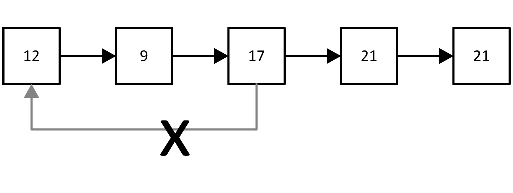
\includegraphics[width=0.5\textwidth]{lineartopology.pdf}
	\caption{A simple left to right linear HMM topology.}
	\label{fig:lineartopology}
\end{figure}

In the first architecture, a HMM for each distinct gesture is created (example: angry-1, angry-2,\ldots, fear-1, fear-2,\ldots,fear-n,\ldots), even though they might represent the same emotion category (example: angry, fear). In this architecture the system is able to distinguish between various forms of gestures through which the same emotion can be identified. If someone is really angry they might point at someone and oscillate their hands toward them in short bursts. If someone is angry and disappointed, they might shrug the shoulders and throw their hands up in the air swiftly. 

In the second architecture, we intend to create a HMM for each distinct emotion (angry, fear,\ldots). In this architecture many similar gestures are grouped together into a single emotion, and some gestures share similar observation sequences, as shown in \ref{fig:multitopology}. HMM topology can be changed depending on the problem being tackled. 

\begin{figure}[htbp]
	\centering
		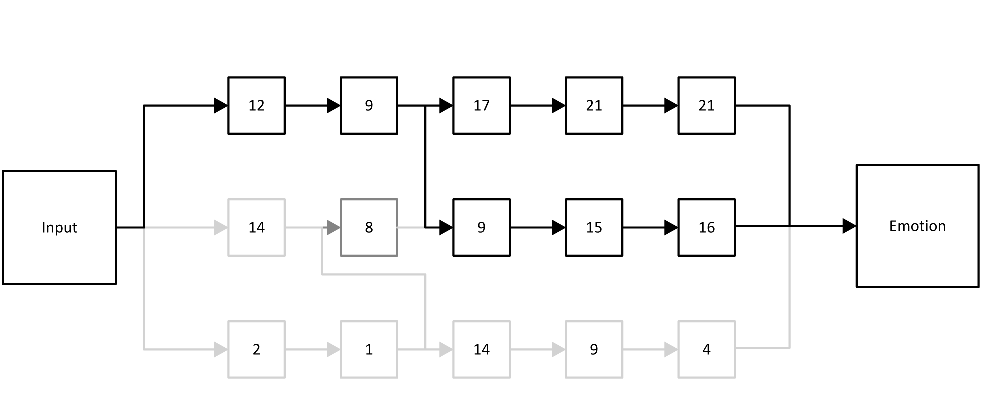
\includegraphics[width=1.0\textwidth]{multitopology.pdf}
	\caption{A multi-tier HMM topology for an emotion.}
	\label{fig:multitopology}
\end{figure}

\section{Data sets} The framework was built by conducting experiments with the UCLIC Affective Posture and Body Motion Database created by Nadia Bianchi-Berthouze and Andrea Kleinsmith\cite{Kleinsmith:2006:CDR:1221613.1222203}. This database contained gestures performed by various actors displaying the \texttt{angry}, \texttt{fear}, \texttt{sad} and \texttt{happy} emotions. The database also captures the cross-cultural variations of the gestures. Each gesture in the database contains approximately 400-1200 frames of data capture. Only a few frames were selected, at equally spaced time intervals to help in loading and reading the data set. The frames contain position coordinates of the points on the actor's body that were tracked using a motion capture system. In each frame 47 3D position coordinates were extracted; examples, include location of left wrist, right wrist, left knee, right knee. 

\begin{figure}[htbp]
  \centering
  \subfloat[Angry]{\label{fig:aff11}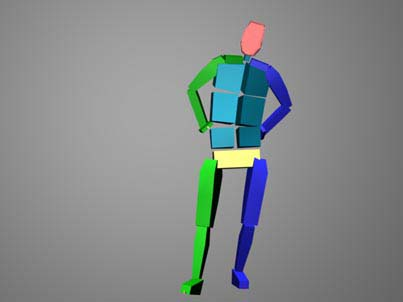
\includegraphics[width=0.50\textwidth]{aff1.jpg}}\hfill
  \subfloat[Happy]{\label{fig:aff12}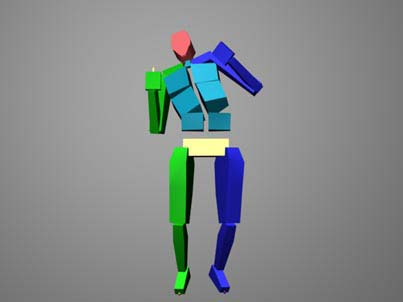
\includegraphics[width=0.50\textwidth]{aff3.jpg}}\hfill
  \caption{Posture samples from UCLIC Affective Posture and Body Motion Database\cite{Kleinsmith:2006:CDR:1221613.1222203}}
  \label{fig:aff1}
\end{figure}

Once the initial framework was developed, and the performance fine-tuned, it was decided that a test should be done on the robustness of the framework. So another data set was obtained from UCLIC Affective Posture and Body Motion Database however this data set contained non-acted\cite{KlEINSMITH_Bianchi-Berthouze_Steed_2011} motion capture data. In the non-acted data set the actors were not acting a specific emotion, rather they were asked to perform a task. Similar to the acted data set, a motion capture system captured the movements of the actor for later analysis. Whilst performing the task the actors expressed various emotions which were categorized into four groups\cite{KlEINSMITH_Bianchi-Berthouze_Steed_2011}: \textit{concentrating} (determined, focused, interested); \textit{defeated} (defeated, give up, sad), \textit{frustrated} (angry, frustrated), and \textit{triumphant} (content, excited, motivated, happy, victory).  However, the data set was not labeled into the above categories when we received them, we classified the data set manually with the following labels instead, \textit{positive}, \textit{negative} and \textit{neutral} emotions. Unlike the acted data set this data set contained Euler joint angles rather than position coordinates. The data set was converted to position coordinates, extracting 23 3D position coordinates on the actor's body. A single data capture in the data set contained approximately 15000-30000 frames, from these frames only a few hundred were extracted that contained a gesture being performed by the actor.

For the final experiment, Xbox Kinect was used for creating a dataset of four different gestures. The four gestures that were performed are \texttt{shurg}, \texttt{shake fist}, \texttt{surprised} and \texttt{thinking}. Only upper body joint positions were captured in the dataset as these gestures primarily exhibited upper body motion. Approximately 10-12 gesture variations of the primary gestures were captured, for a total of 46 gestures. The gestures were performed across a time length of 2-3s, and the sensors captured 3-4 frames per second. 

\subsection*{Features in the data set}
Table \ref{tab:data setfeatures} lists the features that were recorded by the motion capture system in the data sets. Features can be added or removed as necessary to get better results. For example, developing a system that only uses recognizes upper body postures; we can remove features related to the lower body without affecting the results.

% Table generated by Excel2LaTeX from sheet 'Sheet1'
\begin{table*}[htbp]
  \centering
    \begin{tabular}{l|l}
    \toprule
    CSM File (Acted data set)  \\
    \midrule
    Left Front Head  & Left Front Waist  \\
    Left Back Head  & Left Back Waist  \\
    Right Back Head  & Right Back Waist  \\
    Right Front Head  & Right Front Waist  \\
    Top Chest  & Top of Spine  \\
    Center Chest  & Middle of Back  \\
    Left Outer Knee  & Right Outer Knee  \\
    Left Inner Knee & Right Inner Knee \\
    Left Outer Ankle  & Right Outer Ankle  \\
    Left Heel & Right Heel \\
    Left Outer Metatarsal  & Right Outer Metatarsal  \\
    Left Inner Metatarsal & Right Inner Metatarsal \\
    Left Toe  & Right Toe  \\
    Left Shoulder  & Right Shoulder  \\
    Left Outer Elbow  & Right Outer Elbow  \\
    Left Inner Elbow & Right Inner Elbow \\
    Left Wrist Stick End  & Right Wrist Stick End  \\
    Left Wrist Stick Base  & Right Wrist Stick Base   \\
    Left Wrist Inner near thumb & Right Wrist Inner near thumb \\
    Left Wrist Outer opposite thumb & Right Wrist Outer opposite thumb  \\
    Left Hand  & Right Hand  \\
    \midrule
    BVH File (Unacted data set)  \\
	\midrule
		Left Hip	&  Right Hip	\\
		Left Knee&	Right Knee \\
		Left Ankle & Right Ankle \\
		Left Collar & Right Collar \\
		Left Shoulder & Right Shoulder \\
		Left Elbow & Right Elbow \\
		Left Wrist & Right Wrist \\
		Head & \\
		Neck & \\
		\midrule
    Xbox Kinect joint captures  \\
	\midrule
		Left Hip	&  Right Hip	\\
		Left Knee&	Right Knee \\
		Left Ankle & Right Ankle \\
		Left Shoulder & Right Shoulder \\
		Left Elbow & Right Elbow \\
		Left Wrist & Right Wrist \\
		Nexk & \\
		Head & \\
		Spine & \\		
	\bottomrule
	\end{tabular}
	\caption{Feature labels recorded in the motion capture data sets.}
	\label{tab:data setfeatures}
\end{table*}


\section{Feature vector}Elbow angle, position of wrist, knee angle, angle at the hips, head tilt, are some of the data that one needs to assess to distinguish one gesture from another. Together, they form a feature vector. Having the right feature vector is essential in classifying and recognizing gestures. If one has a feature vector consisting of upper body joint positions alone, the accuracy of recognizing gestures that requires having information about the lower body point positions will be low. Likewise, the information in the feature vector is also important, a feature vector consisting of joint points and a feature vector consisting of joint angles might provide different recognition results.

\begin{figure}[htbp]
	\centering
		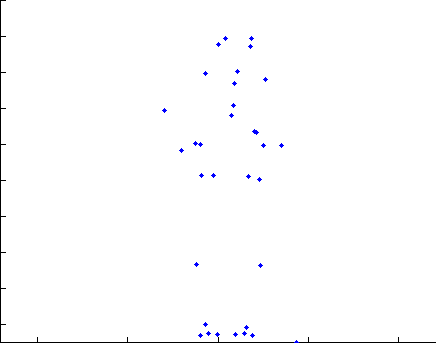
\includegraphics[width=0.65\textwidth]{dimdata.png}
	\caption{Visualization of a dimensioned feature vector (position).}
	\label{fig:dimdata}
\end{figure}

\begin{figure}[htbp]
	\centering
		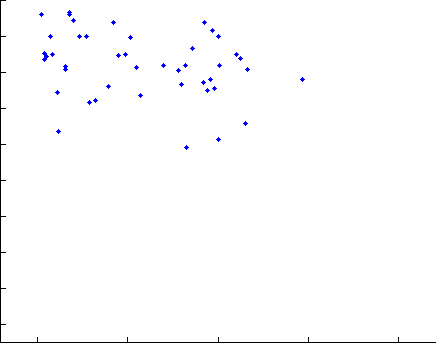
\includegraphics[width=0.65\textwidth]{dimlessdata.png}
	\caption{Visualization of a dimensionless feature vector (velocity).}
	\label{fig:dimlessdata}
\end{figure}

\subsection*{Dimensioned data}
Dimensioned data provide a means to an end in understanding how the HMM framework works in classifying and recognizing sequence of patterns. In the experiments conducted the dimensioned data consisted of having 3D positions of various points of the human body. When these points are plotted for a single frame it is easy to visualize, figure \ref{fig:dimdata}, how the HMM framework works to recognize and classify gestures. However, there are greater disadvantages to using dimensioned data in a classification and recognition algorithm. This data might convey information visually to a human observer, but an algorithm sees no advantage in having dimensioned data. Dimensioned data restricts the algorithm from performing equally well when the input data conveys the same gesture but is performed by a different actor. Different actor's exhibit different dimensioned data for the same gesture, the actor's height, length of arms, and length of legs are all different. Though a human observer is able to filter out these data when we interpret the gesture being performed, an AI algorithm is unable to filter or transform this data in such a way that its recognition and classification is unaffected. 


\subsection*{Dimensionless data}
Dimensionless data play an important role in machine learning, specifically in gesture recognition; it allows data to be generalized for any actor regardless of their physical features. When we compare angry, fear, happy or sad gestures from one actor to another, they will be quite similar when dimensionless data is used. Dimensionless data represent temporal data of a gesture, such as velocity and acceleration of points on a human body, or of joints; essentially data that represents a state in time. Such data is difficult for a human observer to visualize and categorize effectively. Figure \ref{fig:dimlessdata} is the corresponding velocity feature vector of the posture presented in figure \ref{fig:dimdata}.  By observing the velocity of points on a human body one cannot classify the gesture being performed without the help of spatial data. However, this provides no challenge for a machine learning framework, since they will be trained to recognize gestures from this perspective. We realize that gestures are sometimes dependent on speed at which it is being performed; a reactive gesture like fear occurs in a shorter time span than an expressive gesture such as happy, or sad. The temporal pattern recognition of HMM records such anomalies between various gestures during training\cite{Yang_1994_329, 54527}. If someone ducks within a second, it can be said that they reacted to a dangerous situation. If they ducked slowly, they are most likely reacting to a neutral situation. 


\section{Codebook}
Vector quantization plays an important role with any HMM framework, they are necessary to reduce the dimensionality of the feature vector. The generation of a codebook is a vector quantization process. The idea is to take a feature vector and assess all possible ranges across which the feature can have values. Then, this range is quantized, divided into many parts, with some structure. For gesture recognition with motion capture data, two different codebooks techniques are considered in the experiments. Any feature vector considered for training, or classification, is converted into one of the codebook pages that best represent the feature vector.

The first codebook involves the selection of template postures from the training data. These postures were then saved in the template database, which is the codebook. An example of a codebook is shown in figure \ref{fig:codebook1}. This template matching technique is used by \citet{springerlink:10.1007/s00422-004-0516-0} and \citet{springerlink:10.1007/11492429_73}. An advantage to creating such a codebook is that the templates tend to be unique and of value, as it is most likely to be hand-picked by a human. The disadvantage is that if there is a large data set from which the templates need to be chosen from, it will be a tedious task.

The second codebook involves the use of the k-means clustering algorithm to group similar postures together, and these similar postures are put in the same cluster. The k-means algorithm is a common method used in the creation of codebook\cite{Yang_1994_329}. Thus, any gesture that has a posture where the actor is raising their hand would have the same codebook page for that posture. If the number of clusters is large, then variations of the same posture would be spread out, for a small cluster the variations would fall in the same cluster.


\begin{figure}[htbp]
  \centering
  \subfloat[]{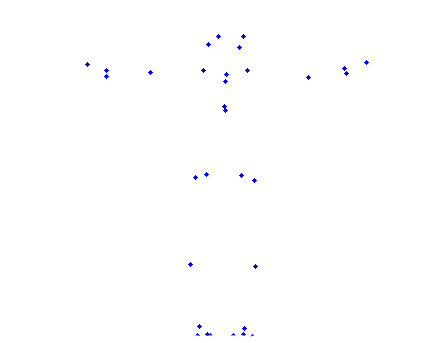
\includegraphics[width=0.33\textwidth]{cb1.png}}\hfill
  \subfloat[]{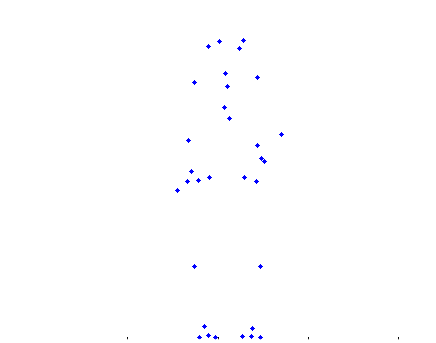
\includegraphics[width=0.33\textwidth]{cb2.png}}\hfill
  \subfloat[]{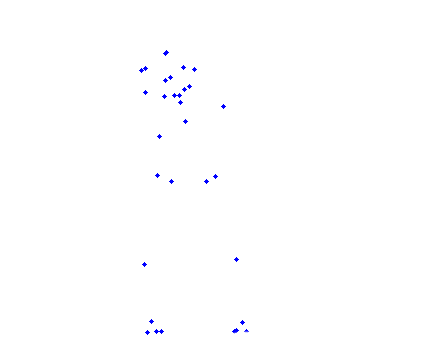
\includegraphics[width=0.33\textwidth]{cb3.png}}\hfill
  \subfloat[]{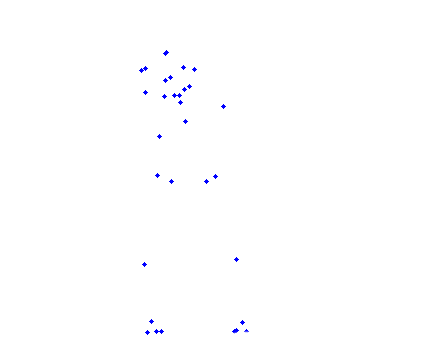
\includegraphics[width=0.33\textwidth]{cb3.png}}\hfill
  \subfloat[]{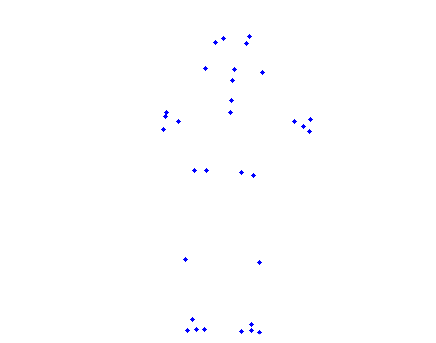
\includegraphics[width=0.33\textwidth]{cb5.png}}\hfill
  \subfloat[]{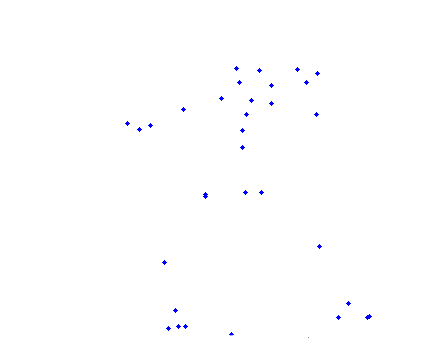
\includegraphics[width=0.33\textwidth]{cb6.png}}\hfill
  \subfloat[]{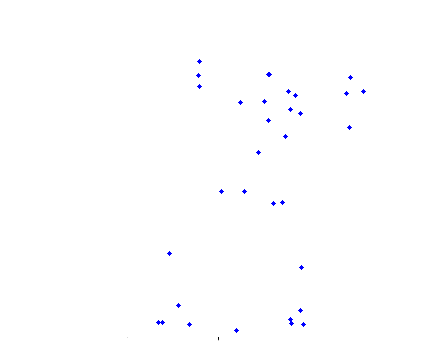
\includegraphics[width=0.33\textwidth]{cb7.png}}\hfill
  \subfloat[]{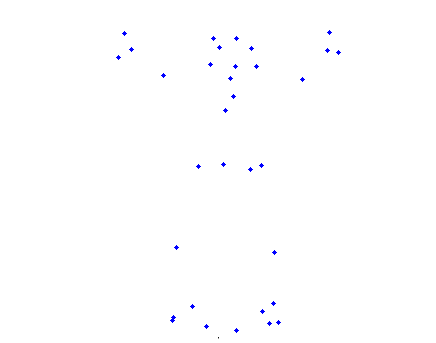
\includegraphics[width=0.33\textwidth]{cb8.png}}\hfill
  \subfloat[]{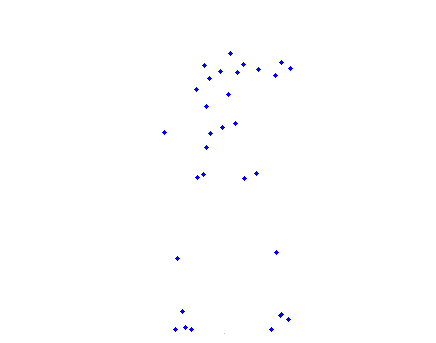
\includegraphics[width=0.33\textwidth]{cb9.png}}\hfill  
  \caption{Dimensioned postures, selected manually, stored in a Codebook.}
  \label{fig:codebook1}
\end{figure}

\chapter{Experiment Results and Analysis}\label{sec:results}
\section{Initial discovery}
The first step in the experiment was to understand how the HMM framework worked, a dimensioned feature vector was used for this purpose. A left-right linear HMM was used for each gesture, as shown in figure \ref{fig:lineartopology}. The codebook vectors were obtained manually. Table \ref{tab:manual} summarizes the results obtained from the various test runs. These experiments used the acted and labeled data set from \citet{Kleinsmith:2006:CDR:1221613.1222203}.

The first type of test consisted of 70 gestures, 35 of which were used for training and 35 for training. We realized that the training sample was quite low, so a second round of tests were conducted which consisted of 90 gestures, 35 were used for testing and 55 for training. Again a third round with even more training data was conducted, with 120 gestures in total, 85 for training and 35 for testing. From the table we can see that the total classified gestures improve as we increase the number of training samples. The number of correctly classified gestures also improves, but at a very low rate. To understand the low classification rate it was necessary to take a closer look at the framework. 
\begin{table*}[htbp]
	\centering
		\begin{tabular}{|l|l|l|l|l|l|l|}
		\hline
		    			& Correctly Classified (\%) & Total Classified & Testing data & Training data & Total Gestures\\
		\hline
			Manual \#1	& 8	(22.8) 	& 10	& 35 &	35 &	70\\
			Manual \#2	& 10 (28.5)	& 24 	& 35 & 	55 &	90\\
			Manual \#3	& 11 (31.1)	& 31 	& 35 & 	85 &	120\\
			K-means 	& 3 (8.5)	& 10	& 35 & 	55 &	90\\
		\hline
		\end{tabular}
	\caption{Recognition}
	\label{tab:manual}
\end{table*}

While training a HMM for a specific gesture, the framework produced the sequence of observations listed in table \ref{tab:fearseq} for one of the fear gestures. Each number corresponds to a page in the codebook, where the content of the page is a single frame of data from the motion capture system. Thus, the frame in page 1 appears after the frame in page 23, similarly the frame in page 10 appears after the frame in page 1, so on. The HMM training algorithm trains a probabilistic model for such a pattern of observation, such that if the sequence in the pattern is altered the HMM would return a low probability for that sequence to appear.

\begin{table*}[htbp]
	\centering
		\begin{tabular}{|l|*{18}{l|}}
		\hline
		 	Fear in Training	&28	&28	&28	&28	&28	&28	&28	&28	&14	&14	&14	&30	&30	&30	&30	\\ \hline
		 	Fear in Testing		&21	&21	&21	&21	&21	&21	&10	&10	&10	&10	&10	&10	&20	&32	&33 \\ \hline
			Angry in Training	&28	&28	&28	&21	&21	&21	&21	&21	&21	&21	&28	&28	&28	&28	&28 \\
		\hline
		\end{tabular}
	\caption{Sequence of observations for an incorrectly classified fear gesture.}
	\label{tab:fearseq}
\end{table*}

Now, we look at the observation pattern for one of the fear gestures in the testing set that was misclassified as one of the angry gestures. When the pattern is compared against the fear gesture in the training set, it is very different. When we compare the pattern to an angry gesture in the training set, half the pattern matches a sequence of observations in the angry pattern. Though only the repetition of the number 21 in the angry gesture matches the fear gesture, the HMM classifies it as angry with a very high probability.

\begin{table*}[htbp]
	\centering
		\begin{tabular}{|l|*{18}{l|}}
		\hline
		 	Angry in Training	&24	&24	&24	&24	&24	&24	&21	&21	&22	&22	&22	&22	&21	&21	&24	\\ \hline
		 	Angry in Testing	&24	&24	&24	&24	&24	&21	&22	&22	&22	&22	&21	&23	&23	&24	&24	\\
		\hline
		\end{tabular}
	\caption{Sequence of observations for a correctly classified angry gesture.}
	\label{tab:angryseq}
\end{table*}

Table \ref{tab:angryseq} displays the observation pattern for a correctly classified angry gesture. Note the similarity of the patterns between the training angry gesture and the testing angry gesture. The HMM classified this as an angry gesture with a very high probability. From these tables we conclude that both, the observation that follows the current observation, and the repetition of the same observation in a sequence plays a key role in determining the outcome of a HMM.

If one were to extract template frames from a training data set of 90 gestures, approximately 1-2 template frames per gesture, we would have approximately 225 templates. This also means that our codebook has 135 pages. A large codebook means a larger training data set is necessary to estimate a large observation probability matrix for our HMM. We quickly realize that many of the gestures share similar postures, a manual selection of templates ensured that the posture selection for codebook pages were unique in nature. Through observations and visual analysis we realized that in our experiments the problem lies in the creation of this codebook. Manual creation of the template frames though accurate was infeasible when the training data set became larger and larger. It was not as straight forward as selecting a few universal template for angry gestures, and use these templates to convert the training data set into a sequence of observation patterns as in tables \ref{tab:fearseq} and \ref{tab:angryseq}. It was necessary to go through each training data set to identify unique gestures, and extract frames from them to properly classify similar gestures. The training data itself contained new patterns that needed to be extracted. 

We introduced a clustering algorithm to replace the manual codebook creation process. The \texttt{k}-means clustering algorithm, creates \texttt{n} clusters and groups similar data together in the \texttt{i}th cluster of the \texttt{n} clusters. The algorithm clusters similar data by calculating the distances of the centroid of the given data, thus data that is closer to each other are grouped in the same cluster. Now, the codebook creation was simplified for a large data set. Table \ref{tab:manual} lists the results of the test runs conducted after using the clustering algorithm for codebook creation. The results are not impressive at all, visual analysis of the codebook vectors and the observation patterns created for each posture tells us why. 

Having a codebook that is as large as 225 pages, even for small variations between two similar gestures the observation sequences are widely different, as in the fear gesture in table \ref{tab:fearseq}. Consider the images in figures \ref{fig:similarcodebook}, they represent figures from codebook pages 2, 11 and 18. Visually they are very similar to each other; however the k-means algorithm clusters them into different pages because of small variations that categorize these images as outliers, such as hip angle, position of wrist, head tilt, and spacing between the feet. These are very subtle from the figures; however the k-means algorithm picks up on these. 

\begin{figure}[htbp]
  \centering
  \subfloat[Codebook Page 2]{\label{fig:page2}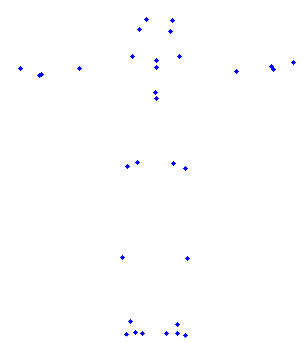
\includegraphics[width=0.30\textwidth]{kms-2.png}}\hfill
  \subfloat[Codebook Page 11]{\label{fig:page11}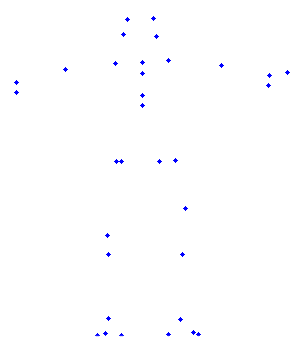
\includegraphics[width=0.30\textwidth]{kms-11.png}}\hfill
  \subfloat[Codebook Page 18]{\label{fig:page18}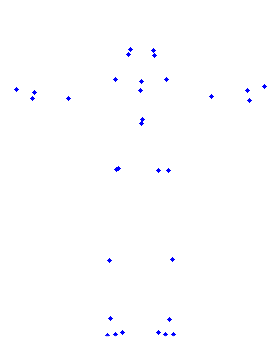
\includegraphics[width=0.30\textwidth]{kms-18.png}}\hfill
  \caption{Similar codebook pages}
  \label{fig:similarcodebook}
\end{figure}

With this in mind, we plotted the postures in the pages listed for the fear gesture, from table \ref{tab:fearseq}; pages 21 and 28 were similar, and pages 14 and 10 were similar. The misclassification in the experiment is caused by such occurrences, of similar postures being classified into different codebook pages. Similar postures are being categorized under different pages because of small variations in position of points on the human body in 3D-space. We suspect that the use of dimensioned feature vectors is causing this, so we proceed by using dimensionless feature vectors.

We also make one final observation about the current architecture. Every gesture has a HMM associated with it even though it might be similar to an existing gesture that has already been trained. This does not pose a problem if every single gesture in the data set were unique. In our data set, the gestures that belong to the \texttt{angry} category is not all unique, many of the gestures are similar with small variations. In a problem that involves humans, whose features and expressions are varied, it is necessary to group up these variations in gestures under a single gesture. Thus, we consider training all unique and non-unique gestures that belong to the \texttt{angry} category under one HMM. If this HMM results in a high probability of a gesture occurring during testing, then it will be classified as \texttt{angry}. This is a multi-tiered HMM topology as shown in figure \ref{fig:multitopology}.

\section{Improving performance}
The initial experiments conducted above have given us important insights into how gesture recognition heavily depends on organizing the codebook pages. The second part of the experiment modified the HMM architecture such that similar gestures were categorized and trained under a single HMM. Thus for a data set that contains four emotions (angry, fear, sad, and happy) four HMMs were created. 
     
\begin{table*}[htbp]
	\centering
		\begin{tabular}{|l|c|c|c|c|}
		\hline
             & Angry & Fear & Happy & Sad \\ \hline
        Angry & 13     & 2    & 0     & 1   \\ \hline
        Fear  & 11     & 7    & 6     & 3   \\ \hline
        Happy & 2     & 1    & 11    & 6  \\ \hline
        Sad   & 3     & 1    & 1     & 19  \\
		\hline
		\end{tabular}
	\caption{Confusion matrix for 3-state HMMs with velocity feature vectors.}
	\label{tab:dim3state}
\end{table*}

Table \ref{tab:dim3state}, displays the confusion matrix for one of the test runs that classified 98\% of the testing data, and 56\% of the testing data were classified correctly with high probability. The test run had a data set of 192 gestures, 93 were used for training the HMMs, and 89 were used for testing. This test run used velocity feature vectors of the training and testing data, for codebook creation and template matching respectively. Note the classification rate is very high, this is caused by the change in the HMM architecture from using one HMM for every gesture to one HMM for every emotion, where similar gestures are grouped together. This change resulted in having a sufficient amount of training data for each HMM, approximately 23 gestures were used to train each of the angry, fear, sad, and happy gestures. The confusion matrix allows us to identify areas where improvements can be made, we note that most of the \texttt{fear} gesture is being misclassified as \texttt{angry}. The only property to control in a HMM model is the number of states associated with it. The results in table \ref{tab:dim3state} are for HMM models with three states (for each emotion). Table \ref{tab:dim4statefear} lists the confusion matrix for a table where the \texttt{angry}, \texttt{happy} and \texttt{sad} HMMs have three states and the \texttt{fear} HMM has four states.   
\begin{table*}[htbp]
	\centering
		\begin{tabular}{|l|c|c|c|c|}
		\hline
             & Angry & Fear & Happy & Sad \\ \hline
        Angry & 5     & 4    & 3     & 4   \\ \hline
        Fear  & 5     & 9    & 9     & 4   \\ \hline
        Happy & 1     & 4    & 9    & 6  \\ \hline
        Sad   & 1     & 2    & 1     & 20  \\
		\hline
		\end{tabular}
	\caption{Confusion matrix where fear HMM has 4-states.}
	\label{tab:dim4statefear}
\end{table*}
We note that the classification of the \texttt{fear} emotion has improved slightly, but the classification of the \texttt{angry} emotion has dropped. Comparing table \ref{tab:dim3state} and \ref{tab:dim4statefear}, the classification of \texttt{happy} emotion has dropped and now the majority of the \texttt{fear} motions are also being classified as \texttt{happy}. We proceed by adding more training data to see if this has any effect. A caveat that needs to be noted here is that, if there are gestures that are unique to a particular emotion that were not being classified properly but now this gesture is in the training data, this gesture will not be tested for in the testing data. 
\begin{table*}[htbp]
	\centering
		\begin{tabular}{|l|c|c|c|c|}
		\hline
             & Angry & Fear & Happy & Sad \\ \hline
        Angry & 4     & 2    & 0     & 0   \\ \hline
        Fear  & 0     & 5    & 2     & 1   \\ \hline
        Happy & 1     & 0    & 4    & 2  \\ \hline
        Sad   & 1     & 2    & 0     & 6  \\
		\hline
		\end{tabular}
	\caption{Confusion matrix for 3-state HMMs with additional training data.}
	\label{tab:dim3statmoredata}
\end{table*}

Table \ref{tab:dim3statmoredata} lists the confusion matrix for which there were 152 gestures for the training data, approximately 38 gestures for each emotion, and 30 gestures for the training data. All the data were classified and it achieved a 63\% correct classification rate. With the caveat, that some unique gestures might not be in the testing data, in mind, we can say in general that higher training data improves the recognition rate of the HMMs. One scenario to think about is how the classification rates are when only two of the emotions are trained and tested for.
\begin{table*}[htbp]
	\centering
		\begin{tabular}{|l|c|c||c|r|}
		\hline
             & Angry & Happy & States & Recognition rate \\ \hline
        Angry & 11     & 11    & 3   & \multirow{2}{*}{71\%} \\ 
        Happy  & 2    & 24   & 4   &  \\ \hline
		Angry & 15     & 7    & 3   & \multirow{2}{*}{78\%} \\ 
        Happy  & 3    & 23   & 3   &  \\ \hline
             & Angry & Sad & \multicolumn{2}{|c|}{}\\ \hline
        Angry & 14     & 6    & 3   & \multirow{2}{*}{81\%} \\ 
        Sad  & 1    & 20   & 3   &  \\ \hline
		Angry & 18     & 2    & 3   & \multirow{2}{*}{83\%} \\ 
        Sad  & 4    & 17   & 2   &  \\ \hline
             & Angry & Fear & \multicolumn{2}{|c|}{}\\ \hline
        Angry & 17     & 4    & 3   & \multirow{2}{*}{66\%} \\ 
        Fear  & 10    & 12   & 3   &  \\ \hline\hline
             & Fear & Happy & \multicolumn{2}{|c|}{}\\ \hline
        Fear & 14     & 4    & 3   & \multirow{2}{*}{72\%} \\ 
        Happy  & 8    & 20   & 3   &  \\ \hline
		Fear & 11     & 7    & 2   & \multirow{2}{*}{74\%} \\ 
        Happy  & 4    & 24   & 4   &  \\ \hline
             & Fear & Sad & \multicolumn{2}{|c|}{}\\ \hline
        Fear & 15     & 9    & 4   & \multirow{2}{*}{77\%} \\ 
        Sad  & 0    & 21   & 3   &  \\ \hline
		Fear & 19     & 5    & 4   & \multirow{2}{*}{85\%} \\ 
        Sad  & 0    & 21   & 4   &  \\ \hline		\hline
             & Sad & Happy & \multicolumn{2}{|c|}{}\\ \hline
        Sad & 14     & 4    & 4   & \multirow{2}{*}{61\%} \\ 
        Happy  & 2    & 13   & 4  &  \\ \hline
		\end{tabular}
	\caption{Confusion matrix for comparison against each emotion.}
	\label{tab:dimemocomp}
\end{table*}

Table \ref{tab:dimemocomp} displays a confusion matrix, recognition rate and the number of states used for each emotion's HMM. We note that when comparing two emotions to each other an average of 15-20\% misclassification rate exists. Table \ref{tab:dimemocomp} also displays improvements on recognition rate when comparing some emotions, for example \texttt{fear} vs. \texttt{sad}. Training the HMMs with 4 states fear and 3 states for sad, a recognition rate of 77\% is achieved, but result is improved upon by training both HMMs with 4 states. Optimization of HMMs for states is an important step in improving the recognition rate. This property not only affects how well the respective gestures are classified (a sad gesture classfied as a sad emotion), but also how other gestures are classified against it (a fear gesture classified as a sad emotion). Improving a classification rate for one gesture might affect the classification rate of another gesture. Thus, when one or more emotions are involved, as in tables \ref{tab:dim4statefear} or \ref{tab:dim3statmoredata}, a balance of states between each individual HMM needs to be achieved.

Figure \ref{fig:rr} displays a graph that shows the recognition rate of an emotion as the number of gestures used in training that emotion are increased. This graph represents recognition rate for the \texttt{Angry} emotion only. Approximately, 32 gestures were used in the training of angry emotion. In the graph, the recognition rate generally improves linearly. There are some outliers, and these outliers are caused by the HMM being unable to converge from the randomized initial probability matrix \cite{5384990}. Figure \ref{fig:rr2} displays how the recognition rate of the entire dataset is affected when the amount of training for a single emotion is varied. We notice that there is approximately a 20\% increase in recognition accuracy; of course most of this is just the angry gestures being classified properly.
\begin{figure}[htbp]
	\centering
		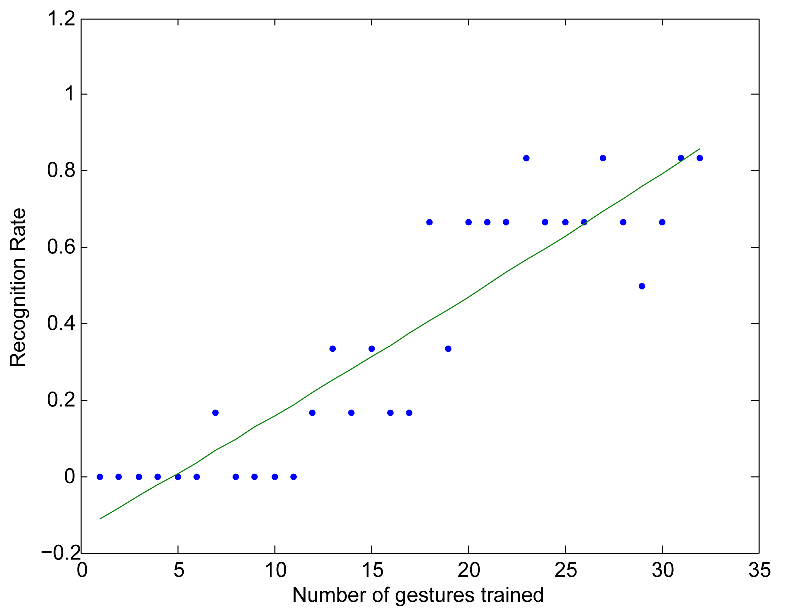
\includegraphics[width=0.65\textwidth]{rr.pdf}
	\caption{Recognition rate (Angry emotion) performance versus number of gestures trained.}
	\label{fig:rr}
\end{figure}

\begin{figure}[htbp]
	\centering
		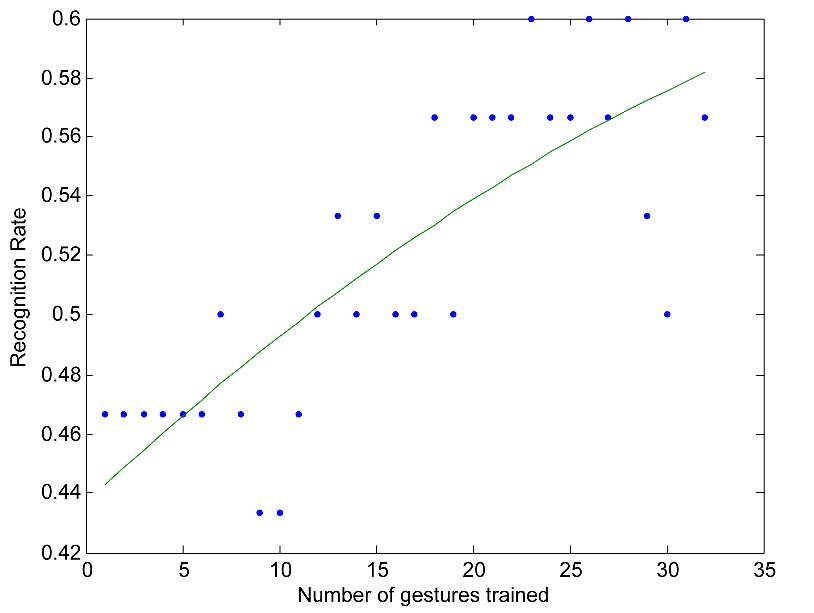
\includegraphics[width=0.65\textwidth]{rr2.pdf}
	\caption{Recognition rate (All emotions) performance versus number of gestures trained.}
	\label{fig:rr2}
\end{figure}

\section{Measured Performance}
It is insightful to look into the overhead experienced by each component of the HMM process. There are two areas where the overhead is significant, when creating a codebook and when training a HMM. Other parts of the process such as extracting feature vectors from the inputs, or even classifying HMM recognition, experience very little overhead. Table \ref{tab:timedperformance} displays the measured performance of the various components of the framework over time. In general, the training data size and the overhead seen are directly correlated. The preprocessing, feature vector extraction, codebook creation and HMM training are \textit{one time} overheads, during the setup phase. When a single new data needs to be trained on top of the existing models, the overhead is very minimal. The performances were measured on an Intel i7, Quad Core CPU, with 8 GB memory.

\begin{table*}[htbp]
	\centering
		\begin{tabular}{|l||r|r|r|}
		\hline
		Training Data Size  		& 10 & 90	& 152 \\ \hline
        Feature Vector Extraction 	&	1.5s & 30.5s     & 44.2s    \\ \hline
        Codebook (k-means)  		& 1s & 25.0s     & 61.2s    \\ \hline
        HMM Training (total) 		&1s & 74.9s     & 37.6s    \\ \hline
        HMM Recognition (total) 	& - & 1.4s     & 1.77 s    \\ \hline
		\end{tabular}
	\caption{Timed performance}
	\label{tab:timedperformance}
\end{table*}

The overhead of the feature vector extraction process is linear in nature, and is very dependent on the process itself. If we are given a data set with spatial positions then algorithmically it is easy to calculate or extract feature vectors from it. If we are given a data set with static images from a camera then the time taken to process the image, isolate human features, and calculate depth and positions becomes significant. The overhead of the codebook creation using the k-means algorithm depends on the length of the feature vector, and the number of feature vectors. As the k-means is an optimization algorithm that iteratively moves data around till the best cluster of data is found\cite{Bottou95convergenceproperties}, it also depends on the values of the feature vector. 

Figure \ref{fig:codebookoverhead1} shows a graphical comparison of the codebook creation time versus the number of features in the feature vector. The amount of time needed to create the codebook using the k-means algorithm increases linearly as the size of the feature vector grows. Figure \ref{fig:codebookoverhead2} shows an alternative comparison of codebook creation time with the number of feature vectors to cluster. Similar to the other graph, the amount of time needed to create the codebook increases linearly as the number of feature vectors to cluster is increased.
\begin{figure}[htbp]
	\centering
		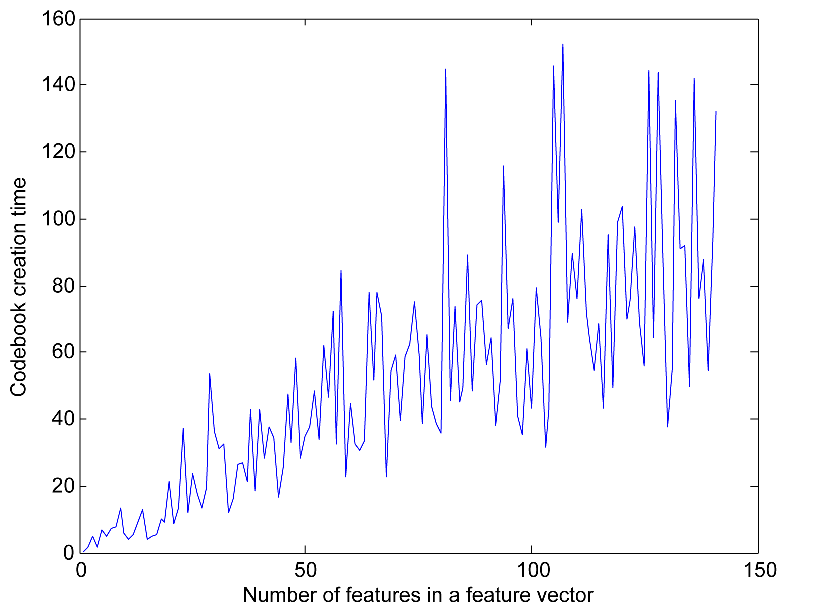
\includegraphics[width=0.65\textwidth]{codebookoverhead.pdf}
	\caption{Graph of codebook creation time (in seconds) versus number of features in a feature vector.}
	\label{fig:codebookoverhead1}
\end{figure}
\begin{figure}[htbp]
	\centering
		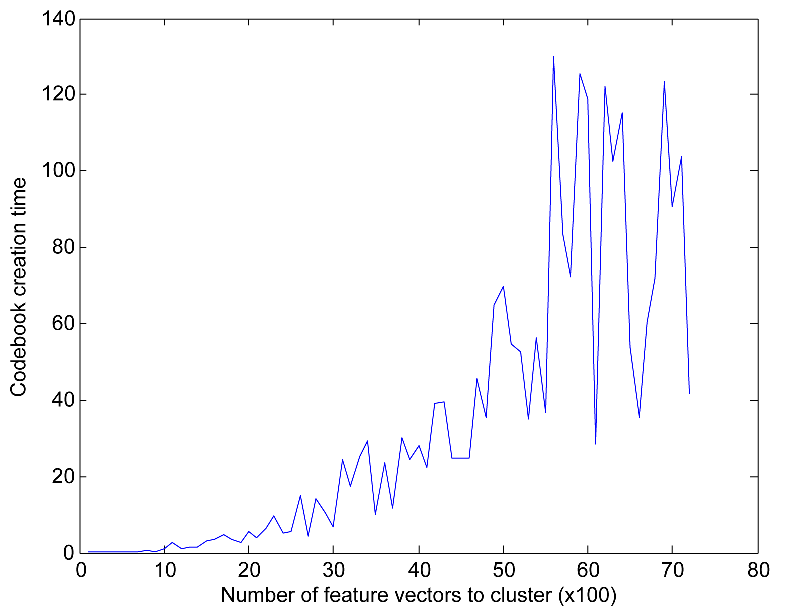
\includegraphics[width=0.65\textwidth]{codebookoverhead2.pdf}
	\caption{Graph of codebook creation time (in seconds) versus number of feature vectors to cluster.}
	\label{fig:codebookoverhead2}
\end{figure}
We notice that figure \ref{fig:codebookoverhead2} contains some outliers where some sets with a higher number of feature vectors tend to have their codebooks created faster than others, this is because of the selection process of the k-means algorithm. If the algorithm makes an initial guess for cluster classification that leads to its convergence criteria faster, then it takes less time for creating the codebooks.

Table \ref{tab:timedperformance} also lists the overhead incurred for HMM training. This is the total training time for all four emotions. Individually, the training of each emotion depends on the number of observation sequence patterns and the rate of convergence of the HMM probability matrices. Figure \ref{fig:trainoverhead} shows a graph of the training times of a HMM as the number of gestures to be trained are increased. Similar to codebook generation, HMM training depends on the convergence of the training algorithm as new gestures are introduced for training. The higher the number of new gestures the longer it takes for training. There are instances when the training time is reduced, that is the convergence of the probability matrix is faster. This is because the gestures are similar to already trained gestures, thus the probability matrix sees less or no improvement at all. Outliers also exist, when the training does not converge to a local optimum we see a large overhead in waiting for the HMM to complete its training.
\begin{figure}[htbp]
	\centering
		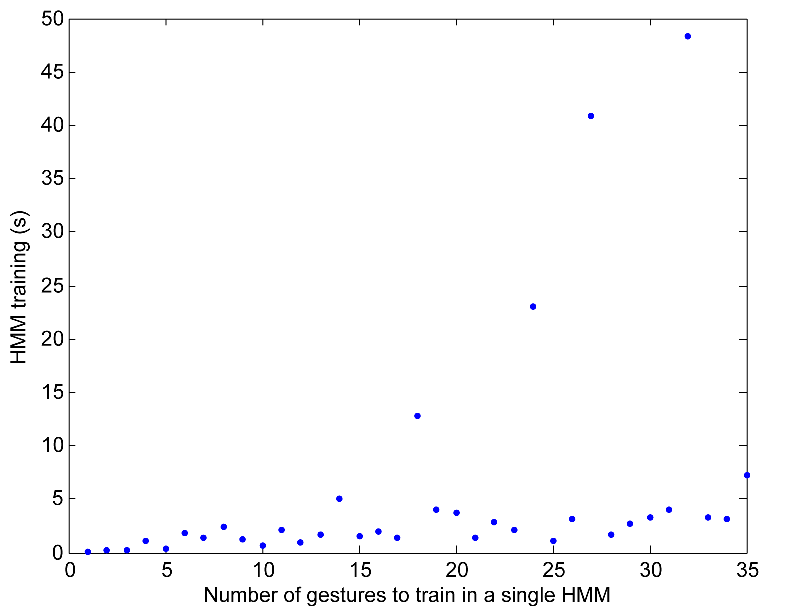
\includegraphics[width=0.65\textwidth]{trainoverhead.pdf}
	\caption{Graph of HMM training time (in seconds) versus number of gestures to train for.}
	\label{fig:trainoverhead}
\end{figure}

\section{Unacted data set}
The experiments that have been discussed until now were performed on an acted data set, where the actor acting the gesture was asked to specifically demonstrate an emotion. A test was also run on an unacted data set from \citet{KlEINSMITH_Bianchi-Berthouze_Steed_2011}. In this data set the actor was asked to perform a task, during this task various emotions were extracted and classified. The idea was to capture the natural essence of an emotion. The gestures were classified into three categories, \texttt{positive}, \texttt{negative}, and \texttt{neutral}. A \texttt{positive} emotion consisted of content, excited, motivated, happy or victory gestures, while a \texttt{negative} emotion consisted of defeated, give up, sad, angry, and frustrated gestures. All other gestures were considered \texttt{neutral}. Even for a human observer it was difficult to label the data set with one of the emotions, thus training a HMM to detect and recognize such gestures would be a test in robustness.

\begin{table*}[htbp]
	\centering
		\begin{tabular}{|l|c|c|c|c|}
		\hline
             & Positive & Negative & Neutral \\ \hline
        Positive & 6     & 1    & 1     \\ \hline
        Negative  & 2     & 3    & 1      \\ \hline
        Neutral & 2     & 2    & 11     \\ \hline
		\end{tabular}
	\caption{Confusion matrix for the unacted data set.}
	\label{tab:unactedconfuse}
\end{table*}

From the tests performed on the acted data set, we see that a dimensionless velocity feature vector with one HMM for each emotion gave us better performance. We apply the same preference towards training and testing the unacted data set. Also, this data set had a smaller feature vector than the acted data set, as displayed in table \ref{tab:data setfeatures}. Table \ref{tab:unactedconfuse} displays the confusion matrix for the unacted data set. A total of 64 gestures were extracted and labeled manually from the data set, of which 33 was used for training the HMMs, and 31 for testing. It is important of to note the distribution of the emotions in the data set. Out of the labeled gestures, 19 were labeled as \texttt{positive}, 17 as \texttt{negative} and 28 as \texttt{neutral} gestures. The framework recognized 61\% of the gestures correctly. The \texttt{positive} and \texttt{negative} HMMs used 2 states while 3 states were used for the \texttt{neutral} HMM.
\begin{table*}[htbp]
	\centering
		\begin{tabular}{|l|c|c|c|c|}
		\hline
             & Positive & Negative & Neutral \\ \hline
        Positive & 3     & 1    & 0    \\ \hline
        Negative  & 0     & 2    & 3      \\ \hline
        Neutral & 0     & 1    & 4     \\ \hline
		\end{tabular}
	\caption{Confusion matrix for the unacted data set.}
	\label{tab:unactedconfuse2}
\end{table*}

A modified test was run to see how additional training data affects the classification results; 49 gestures were used for training, and 15 were used for testing. Table \ref{tab:unactedconfuse2} displays the results of the test. We note that in both cases (tables \ref{tab:unactedconfuse} and \ref{tab:unactedconfuse2}) the \texttt{negative} emotion is performing poorly. The tests did not use a sufficient amount of gestures for training to conclude the reasons behind the misclassification concretely. 60\% of the testing data was classified correctly. Thus we see no improvement in adding more training data in this case, but an observation to note was that only 2 additional \texttt{negative} gestures were added to the training data in the modified test, as more \texttt{negative} gestures were unavailable.

The purpose of these tests were to determine the robustness of the HMM framework for recognizing gestures under different circumstances (acted, or unacted). From the results above we can safely conclude that the HMMs are quite robust to adapt to situations as long as sufficient training is provided.

\section{Xbox Kinect data set}
A final experiment was performed with motion captured data from Xbox Kinect. This was a custom experiment to test the framework's performance with Xbox Kinect data capture, also acted as a sanity check. Brian was to be outfitted with a Kinect camera to capture user interactions, as they are interacting with the social robot. When a person enters the Kinect's view, it starts calibrating joint locations on the user for tracking in real time. This provides us with joint spatial data, table \ref{tab:data setfeatures} shows the list of features captured by the device.

The code that was used to capture data from the Kinect provided us with 3-4 frames per second. We believe that the code could be optimized further to provide us with a higher frame rate. However, 3-4 frames per second were more than sufficient to distinguish the four gestures that were performed for training, testing and classification. The four gestures that were performed are \texttt{shurg}, \texttt{shake fist}, \texttt{surprised} and \texttt{thinking}. Note that we have switched from classifying into emotions labels to classifying into gesture labels; this was due to the limited scope of the experiment. However, we follow a similar setup that ensures that the same steps for emotion label classifications are applied. Even though we have four gestures, each gesture was performed 10-12 times, that is there were 10-12 variations of the same gesture to give us a total of 46 gestures. We consider \texttt{shurg}, \texttt{shake fist}, \texttt{surprised} and \texttt{thinking} as emotion labels for the purpose of this experiment. 

\begin{figure}[htbp]
  \centering
  \subfloat[]{\label{fig:f11}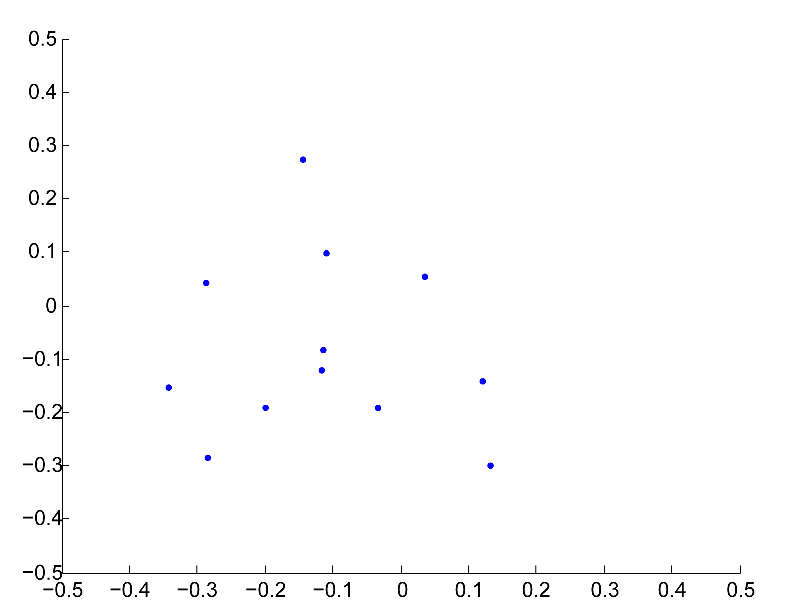
\includegraphics[width=0.50\textwidth]{xbox-think-1.pdf}}\hfill
  \subfloat[]{\label{fig:f12}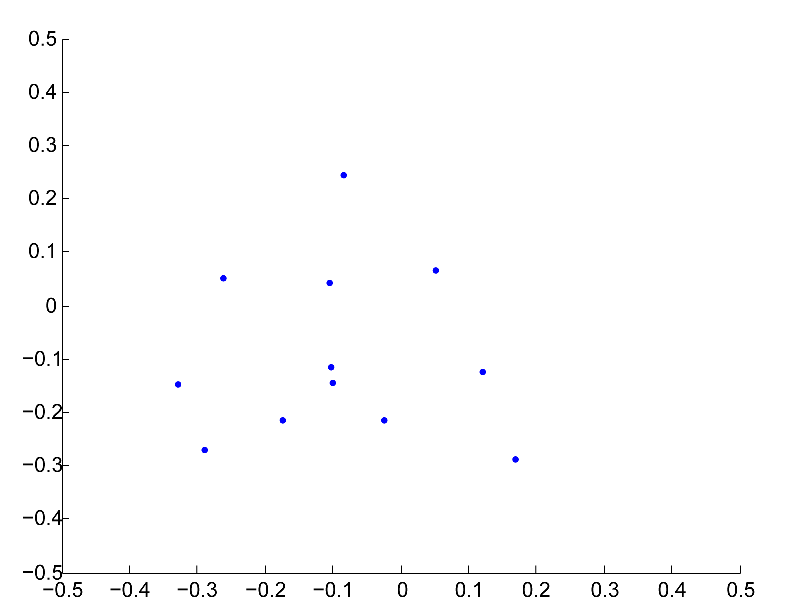
\includegraphics[width=0.50\textwidth]{xbox-think-2.pdf}}\hfill
  \subfloat[]{\label{fig:f13}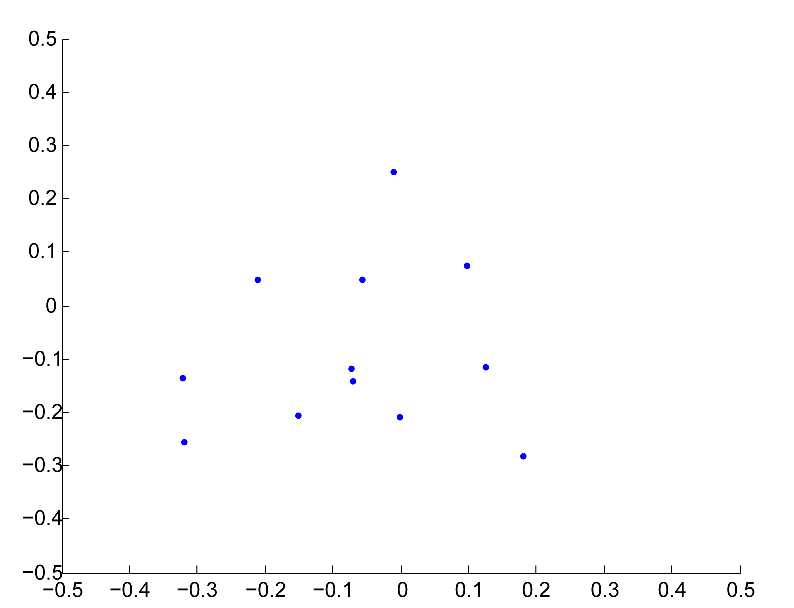
\includegraphics[width=0.50\textwidth]{xbox-think-3.pdf}}\hfill
  \caption{Sequence of posture progression in a \texttt{thinking} gesture}
  \label{fig:xboxthink}
\end{figure}

\begin{figure}[htbp]
  \centering
  \subfloat[]{\label{fig:f21}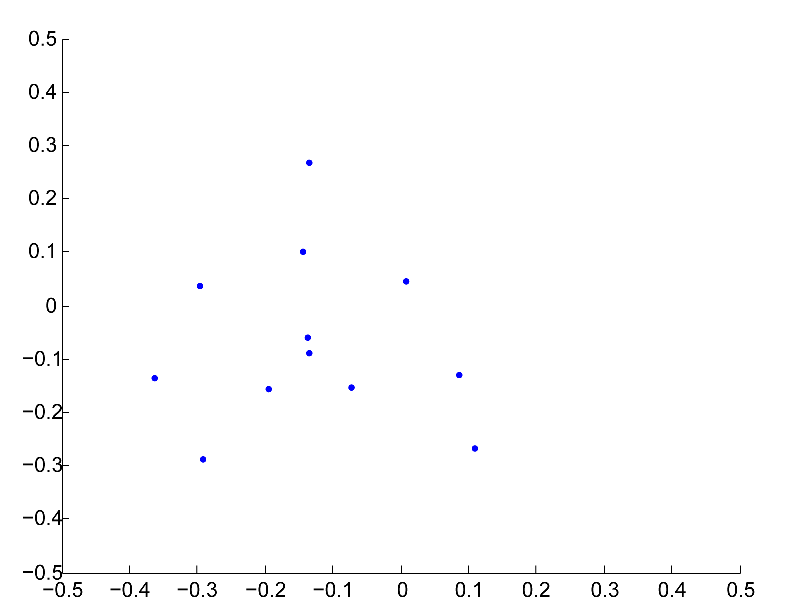
\includegraphics[width=0.50\textwidth]{xbox-shrug-1.pdf}}\hfill
  \subfloat[]{\label{fig:f22}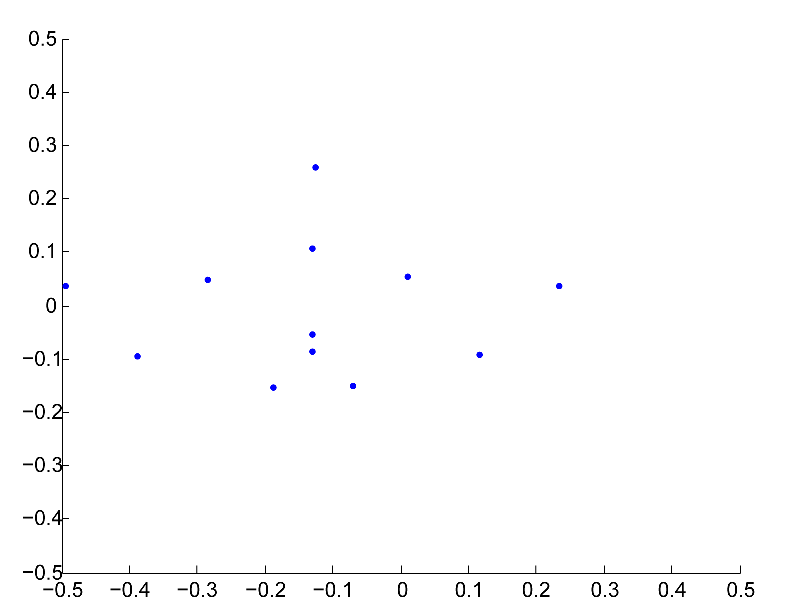
\includegraphics[width=0.50\textwidth]{xbox-shrug-2.pdf}}\hfill
  \caption{Sequence of posture progression in a \texttt{shrug} gesture}
  \label{fig:xboxshrug}
\end{figure}
Figure \ref{fig:xboxthink} displays three of the frames captured in the thinking gesture. Note the subtle changes in the position of the head and the hands. Figure \ref{fig:xboxshrug} displays two of the frames captured in a shrug gesture. Note the change in position of the hands. Something to realize is the power of HMMs to detect and appropriately classify these subtle changes in postures among different gestures.

Once the data was captured, the same steps as the other experiments were followed to extract velocity feature vectors and the k-means algorithm was used to create a codebook. With the training observations created, the HMM was trained for each emotion label with the corresponding gestures. The initial test run consisted of 22 training data and 24 testing data. Table \ref{tab:xboxdim3state1} contains the confusion matrix for the 3-state HMM that was trained and tested against. 
\begin{table*}[htbp]
	\centering
		\begin{tabular}{|l|c|c|c|c|}
		\hline
             & Shrug & Surprised & Thinking & Shakefist \\ \hline
        Shrug 		& 4     & 0    & 0     & 0   \\ \hline
        Surprised 	& 0     & 2    & 6     & 0   \\ \hline
        Thinking 	& 1     & 0    & 1     & 0  \\ \hline
        Shakefist   & 6     & 0    & 2     & 0  \\
		\hline
		\end{tabular}
	\caption{Confusion matrix for 3-state HMMs with velocity feature vectors for Xbox Kinect data set.}
	\label{tab:xboxdim3state1}
\end{table*}
The classification rate for this test run was 59\%, 13 out of 22 gestures in the testing data set were classified correctly. From table \ref{tab:xboxdim3state1} we notice that the majority of the \texttt{surprised} and \texttt{shake fist} gestures are being misclassified. The \texttt{shurg} gesture has a 100\% classification rate, but the \texttt{shake fist} gesture is being misclassified mostly as the \texttt{shrug} gesture. To identify the cause of miss classification we review the contents of the shrug and shake fist gestures visually. Visually the gestures are quite different, as the shrug was dependent primarily on shoulder movements, while the shake fist was dependent on a moving hand in front of the actor. Next we analyze the gestures in the training data set, and found that only one shake fist was being used to train the HMM. As such the variations in this gesture were not being captured.

The second test runs involved shifting more data from the test data set to the training set. The gestures were shuffled and randomly selected for testing and training. It was also ensured that sufficient amount of gestures were available to provide training for each emotion label. For training 31 gestures were used, while 15 gestures were used for testing. Similar to the first test run, a 3 state HMM for each emotion label was trained. Table \ref{tab:xboxdim3state2} displays the confusion matrix of this run. 
\begin{table*}[htbp]
	\centering
		\begin{tabular}{|l|c|c|c|c|}
		\hline
             & Shrug & Surprised & Thinking & Shakefist \\ \hline
        Shrug 		& 3     & 0    & 0     & 1   \\ \hline
        Surprised 	& 0     & 3    & 1     & 0   \\ \hline
        Thinking 	& 0     & 2    & 2     & 0  \\ \hline
        Shakefist   & 0     & 0    & 0     & 3  \\
		\hline
		\end{tabular}
	\caption{Confusion matrix for 3-state HMMs with velocity feature vectors for Xbox Kinect data set.}
	\label{tab:xboxdim3state2}
\end{table*}
Out of the 15 gestures, 12 were classified correctly giving us a recognition rate of 80\%. We notice that the shake fist and surprised gesture recognition has improved significantly from the first run. This leads us to the conclusion that having a lack of necessary training data will result in over fitting of the observation sequence probabilities in a HMM. 

\subsection*{Noise variations}
We perform one last experiment with this data set to see how the recognition results are affected with noise. The data set was divided into two, one of which was modified with noisy values. This simulates a random noise disturbance in the motion capture system. Both sets of data were shuffled and re-divided into test and training data sets randomly. This time we trained the existing HMMs that were trained for the previous test run. The difference being instead of the random initial probability matrices, we start with an existing probability matrix from the previous run. Similar to the last experiment, 31 gestures were used for training and 15 gestures were used for testing. Table \ref{tab:xboxdim3state3} displays the confusion matrix for this test run. The test run achieved a correct classification rate of 73\%. 
\begin{table*}[htbp]
	\centering
		\begin{tabular}{|l|c|c|c|c|}
		\hline
             & Shrug & Surprised & Thinking & Shakefist \\ \hline
        Shrug 		& 4     & 0    & 0     & 0   \\ \hline
        Surprised 	& 0     & 2    & 2     & 0   \\ \hline
        Thinking 	& 0     & 1    & 3     & 0  \\ \hline
        Shakefist   & 1     & 0    & 0     & 2  \\
		\hline
		\end{tabular}
	\caption{Confusion matrix for 3-state HMMs with noisy Xbox Kinect data set.}
	\label{tab:xboxdim3state3}
\end{table*}
To improve the misclassifications we would need to provide more training data, or work on optimizing the HMM parameters, such as the probability transition matrix, emission probability matrix, or the number of states allowed in a gesture. One can assume that as various new gestures are trained the performance would drop, as there is a higher chance of confusion between the various gestures. Overall, these results tell us of the success of the experiment in implementing it for use with Xbox Kinect. Assuming we provide sufficient training for each emotion or gesture that needs to be classified, HMMs are quite robust to variations, very easy for training and adaptation. 

\chapter{Future direction}
In the experiments detailed in this report, many performance improvements have been made across the components described above. Kkeeping in focus the applications of HMM, there is plenty of room for growth in optimizing the components further before we debug the theory behind HMM for improvements. Any future research in gesture recognition using HMMs should focus on obtaining better feature vectors. The velocity feature vectors provided us with sufficient performance improvement in the experiments, we suspect that a hybrid feature vector with velocities, and angles, would give us even better performance. Employment of a better algorithm for codebook creation would also improve the performance of HMM framework recognition significantly, as the codebooks are the basis of the symbols in the observation sequences. We believe that we have explored the best options for HMM topology, and it should of less concern in further work.

The next steps in using the results from the experiments in this report would be to implement HMM gesture recognition on to Brian's\cite{dmcoll} architecture to capture body postures in a real-time interaction with users, and classify them. However, before that can be done a study needs to be conducted to train various gestures that the social robot would see. The data sets in the literature do not provided a sufficient variety of gestures that would relate to an elderly interacting with a robot. Thus, such a data set needs to be collected.

\chapter{Conclusion}\label{sec:conclusion}
In this report, we have demonstrated the application of Hidden Markov Models (HMMs) to recognize gestures in motion captured data. The existing works demonstrate how HMMs are very applicable in the field of gesture recognition because of their ability to train and recognize over spatio-temporal data. We start by discussing the process involved in using HMMs for gesture recognition. Then we discuss in detail some of the components related to the architecture of the overall recognition process in chapter \ref{sec:overllprocess}. 

We identify and discuss four key components in the framework: HMM topology, feature vector, data sets, and the codebook in chapter \ref{sec:fwc}. We propose a linear HMM topology and a multi-tier linear HMM topology. We identified the data sets and the purpose of each data set in the experiment. We explore feature vector selection, and identify the importance of dimensionless feature vectors. And finally, we discuss codebook construction by the use of template matching, and alternatively by applying a k-means algorithm.

The initial discovery phase of the experiment analyzed the observation sequences and determined the cause of poor performance. We determined the cause of misclassification of gestures in the recognition process, and the steps necessary to improve it. We also analyzed how the codebook played an important role in HMMs. It was also established that the manual selection of template database is not feasible, as the data size increased. Later, by using a dimensionless feature vector and a multi-tier architecture for classifying similar gestures into emotions, we achieved a gesture recognition rate of 63\%. We test the robustness of the framework to be able to adapt and perform equally well for a different data set. In this final experiment the framework achieved a recognition rate of 60\%. Then we conclude the experiments with a final test, by using an Xbox Kinect, to capture four simple gestures and classify them. The framework achieved a 75-80\% recognition rate in this experiment.

The report has provided a detailed account of the components and the analysis of the framework (process) involved in using HMMs for recognizing gestures in motion capture data. Achieving a 63\% recognition rate; by supplying sufficient and related, training data and tuning HMM properties specifically for recognizing emotions, an even higher recognition rate could be achieved.

\bibliographystyle{unsrtnat}
\nocite{*}
\bibliography{biblio}
\end{document}

